\documentclass[a4paper, 11pt]{article}
\usepackage[utf8]{inputenc}
\usepackage[ngerman]{babel}
\usepackage{graphicx}

\usepackage{url}




\begin{document}

\author{Joachim Leiser}
\title{Entwicklung eines Rahmenwerks zur Realisierung von Videospielklassikern: Pac-Man betreut von Prof. Dr. Christian Pape}
\date{07.10.2016}
\maketitle

\pagebreak

\textbf{Abstract:}



\tableofcontents

\pagebreak

\section{Vorwort} %Worte zur Arbeit im Allgemeinen.

Dies ist eine Projektarbeit im Rahmen des Informatikstudiums an der Hochschule Karlsruhe - Technik und Wirtschaft. Sie wird betreut von Prof. Dr. Christian Pape. Das Thema ist "`Entwicklung eines Rahmenwerks zur Realisierung von Videospielklassikern: Pac-Man"'. Die Arbeit ist aufgeteilt in die Entwicklung des Rahmenwerks und die Entwicklung des Videospiels Pac-Man. Das Rahmenwerk wird in einer Zusammenarbeit mit den Studierenden Christian Modery und Angelo Douvere in der Programmiersprache C++ und dem Framework OpenGL entwickelt. Das Videospiel Pac-Man wird mithilfe des Rahmenwerks in Einzelarbeit entwickelt. Das Videospiel wird in englischer Sprache umgesetzt.



\section{Spezifikationen des Videospielklassikers Pac-Man}
Hier werden die Anforderungen und Regeln des Spiels Pac-Mans festgelegt.

Pac-Man ist ein Arcade- und Videospiel, dass ursprünglich im Juli 1980 in Japan von der Firma Namco unter dem Namen Puck-Man veröffentlicht wurde\cite{WikiPacMan}. 1981 wurde das Spiel in den USA von Midway Games mit dem Namen Pac-Man veröffentlicht. Das Spiel handelt vom gleichnamigen Charaktär Pac-Man, einer gelben Kugel mit einem Mund, die versucht ein zweidimensionales Labyrinth aus "`Dots"' und "`Energizern"' zu fressen, um in das nächste Level aufzusteigen. Dabei wird er von "`Ghosts"' gejagt, welche mit jedem Level klüger werden. Allerdings ist Pac-Man in der Lage für kurze Zeit den Spieß umzudrehen, indem er einen "`Energizer"' frisst. Daraufhin sind die "`Ghosts"' für kurze Zeit geschwächt und für Pac-Man essbar. Alles was Pac-Man isst gewährt ihm Punkte. Ziel des Spiels ist es, als Pac-Man so viele Punkte wie möglich zu verdienen.


\begin{figure}[ht!]
	\centering
	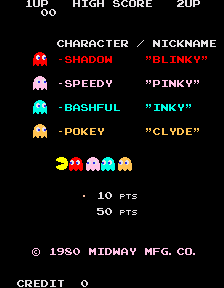
\includegraphics[scale=1]{PacManUebersicht}
	\caption{Geister\cite{MuseumPacMan}}
	\label{PacManGeister}
\end{figure}

\begin{figure}
	\centering
	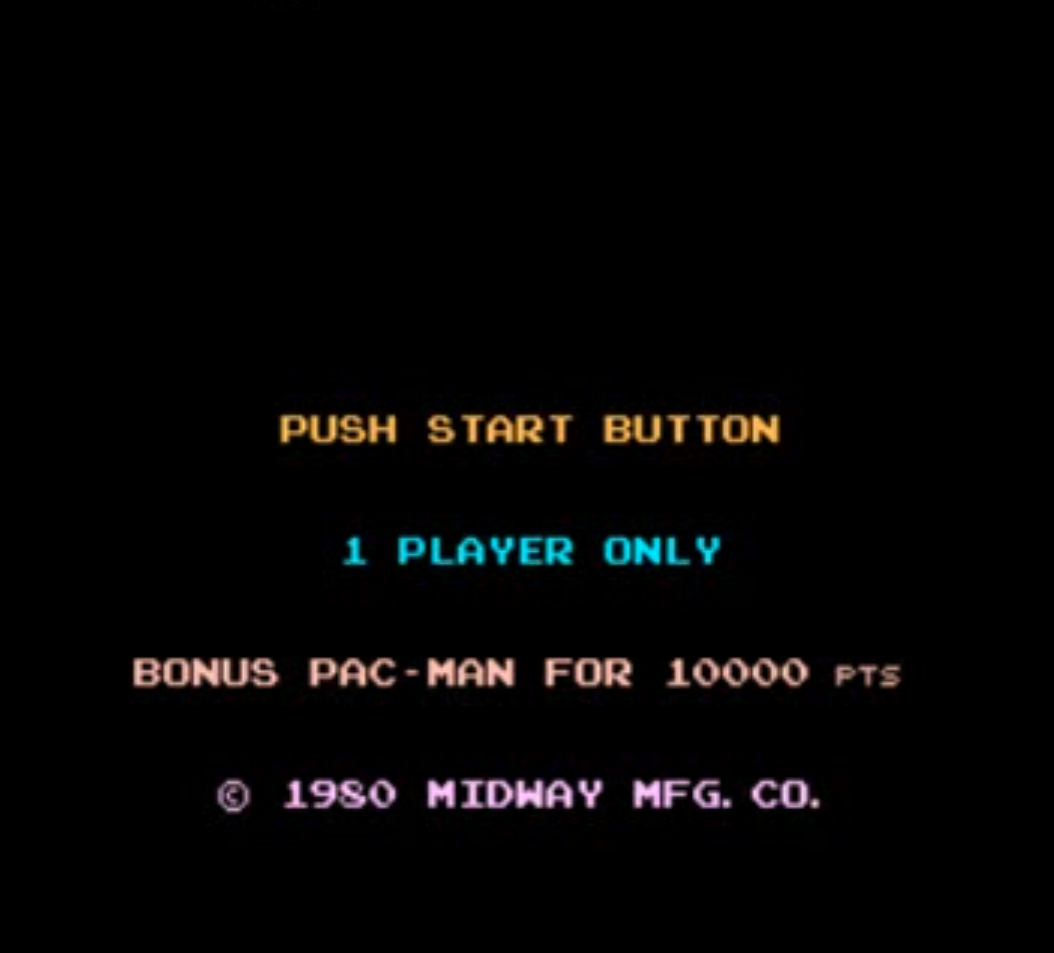
\includegraphics[scale=0.3]{PacManPushStartButton}
	\caption{Startbildschirm\cite{YoutubePacMan}}
	\label{PacManPushStartButton}
\end{figure}

\begin{figure}[ht!]
	\centering
	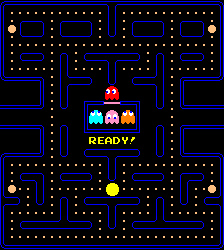
\includegraphics[scale=1]{PacManStartPic}
	\caption{Spielfeld zu Beginn\cite{MuseumPacMan}}
	\label{PacManStart}
\end{figure}

\subsection{Ziel}
Ziel des Spiels ist es eine höchstmögliche Punktzahl zu verdienen. Dabei gibt es nach oben kein Limit. Pac-Man hat auf seiner Reise durch das Labyrinth drei Leben. Wobei er nach $10000$ Punkten ein Bonusleben erhält. Das Spiel ist vorbei wenn sein Leben auf Null fällt.  

\subsection{Menü}
Abb. \ref{PacManGeister} ist der Standby Bildschirm des Spiels. Dabei läuft in einer Animation Pac-Man mit den Geistern im Schlepptau von rechts nach links. Nachdem diese den Bildschirm über den linken Rand verlassen, kehren diese von dort zurück von links nach rechts. Die Geister sind nun dunkelblau wie von einem "`Energizer"'. Pac-Man frisst die Geister einer nach dem anderen auf. Danach startet die Animation von neuem. 
Nach einem Tastendruck erscheint ein Bildschirm wie in Abb. \ref{PacManPushStartButton}. Mit einem weiteren Tastendruck beginnt das Spiel. Nachdem das Spiel beendet wurde kehrt Pac-Man in den Startbildschirm zurück. Bei längerer Inaktivität wird der Standby Bildschirm angezeigt.

\subsection{Level}
Jedes Level sieht zu Beginn aus wie in Abb. \ref{PacManGeister}. Wenn ein Level abgeschlossen wurde, also alle "`Dots"' und "`Energizer"' gefressen wurden, startet das nächste. Mit jedem Level wird das Spiel schwieriger. D.h. die "`Ghosts"' werden klüger. Allerdings gibt es, egal wie hoch das Level auch ist, immer eine Route mit der man das Level gewinnen kann. Theoretisch sollte die Anzahl an Leveln unendlich sein. Praktisch trat im Original ein Bug in Level 256 auf. Durch einen Speicherüberlauf wurde die rechte Hälfte des Spielfelds vom falschen Speicherort gelesen. Damit war das Level auf der rechten Seite nicht sichtbar und das Spiel somit unspielbar.

\subsection{Objekte}
Auf dem Spielfeld sind 240 "`Dots"' und vier "`Energizer"' die Pac-Man einsammeln muss um in das nächste Level zu gelangen. Gelegentlich erscheint in der Mitte des Feldes direkt unter dem kleinen Raum für eine kurze Zeit eine Frucht, die Pac-Man für Bonuspunkte einsammeln kann. Pac-Man sammelt Objekte auf indem er sich auf dasselbe Feld wie ein sammelbares Objekt bewegt. Wenn Pac-Man einen "`Energizer"' frisst werden alle lebenden Geister für eine gewisse Zeit geschwächt und damit dunkelblau. Solange die Geister geschwächt sind, sind sie für Pac-Man ess- bzw. sammelbar. Kurze Zeit bevor die Geister sich erholen blinken sie abwechselnd weiß und dunkelblau. Wenn ein Level abgeschlossen wird startet das nächste wieder mit allen Objekten intakt und allen Charaktären an ihrer jeweiligen Startposition.

\subsection{Fortbewegung}
Figuren können sich durch das Raster von Feld zu Feld bewegen, wobei Wände nicht passiert werden dürfen. Das Feld ist fest vorgegeben und sieht aus wie in Abb. \ref{PacManStart}. Pac-Man kann sich nur horizontal oder vertikal bewegen. Dasselbe gilt für die "`Ghosts"', wobei diese vom Spiel gesteuert werden. Die "`Ghosts"' können sich außerdem nach einer kurzen Wartezeit im Raum in der Mitte sich durch die rosa Tür bewegen. Wenn eine Figur das Spielfeld verlässt, betritt sie es im selben Moment auf der gegenüberliegenden Seite.

\subsection{Eingabe}
Da Pac-Man ursprünglich ein Arcade-Game war, wurde es mit einem Joystick gespielt. Auf Portierungen für den PC werden normalerweise die Pfeiltasten zur Steuerung verwendet.

\subsection{"`Ghosts"'}
Auf Pac-Mans Reise durch das Labyrinth wird er von den 4 Geistern Shadow (Blinky), Speedy (Pinky), Bashful (Inky) und Pokey (Clyde) verfolgt. Diese sind in Abb. \ref{PacManGeister} zu sehen. Jeder Geist hat eine andere Eigenschaft. Speedy ist schneller als alle anderen. Shadow ist immer dicht hinter Pac-Man und schwer abzuschütteln. Bashful ist sehr schüchtern und wird vor Pac-Man sogar wegrennen. Pokey wird sein bestes geben Pac-Man zu fangen, aber er ist langsamer als alle anderen. Wenn Pac-Man mit einem der Geister kollidiert stirbt er. Aber wenn Pac-Man einen "`Energizer"' frisst, färben sich die Geister kurze Zeit dunkelblau. In dieser Zeit isst Pac-Man die Geister bei einer Kollision. Kurz bevor die Geister wieder normal werden, blinken sie weiß und dunkelblau. Von Geistern die gefressen wurden bleiben nur die Augen übrig. Diese bewegen sich zum Mittelpunkt des Spiels wo sich die Geister regenieren. Tote Geister interagieren in keiner Weise mit Pac-Man oder anderen Geistern. 

\subsection{Punkte}
Sammelbare Objekte geben Punkte wenn sie aufgesammelt werden. In Tabelle \ref{table1} ist zu sehen, welches Objekt welche Anzahl Punkte gibt. Die gesammelten Punkte werden aufsummiert und ergeben den "`Score"' bzw. Punktestand des Spiels der über dem Spielfeld eingeblendet wird. Wenn Pac-Man Geister frisst, erhält er Punkte je nachdem welche Anzahl Geister er seit dem letzten "`Energizer"' gefressen hat. Für den Ersten gibt es 200, für den Zweiten 400, für den Dritten 800 und für den Vierten 1600 Punkte. Nach $10000$ Punkten gibt es ein Bonusleben. 

\subsection{Sound\cite{SoundPacMan}}
Für Pac-Man gibt es verschiedene Soundeffekte und eine Hintergrundmusik. Diese sind mit 8-Bit Musik realisiert worden. Es gibt jeweils einen Soundeffekt für folgende Aktionen

\begin{itemize}
\item Intro
\item Pac-Man Mampfer
\item Frucht essen
\item "`Ghost"' essen
\item Extra Pac-Man
\item Intermission
\item Tod
\end{itemize}

Die Soundeffekte sind unter \url{http://www.classicgaming.cc/classics/pac-man/sounds} zu finden.

\subsection{Animationen}
Es gibt Animationen zwischen ein paar Leveln um den Spieler zu amüsieren. Nach dem zweiten Level gibt es eine in der Pac-Man sich über einen schwarzen Bildschirm von rechts nach links bewegt. Dabei wird er vom roten Geist Shadow verfolgt der langsam aufholt. Kurz bevor Shadow Pac-Man einholt, erreichen die Beiden den linken Bildschirmrand und verlassen ihn. Kurz darauf bewegt sich Shadow nun wie durch einen "`Energizer"' blau gefärbt von links nach rechts über den Bildschirm. Dabei wird er von Pac-Man, der nun doppelt so groß erscheint, verfolgt. Shadow wird in der Mitte des Bildschirms von Pac-Man gefangen und gefressen. 

\begin{table}[ht!]
	\centering
	\begin{tabular}{|l|l|}
	\hline
	Objekt & Punkte \\ \hline 
	\hline
	Dot	& 10  \\ \hline
	Energizer & 50 \\ \hline
	Cherry & 100 \\ \hline
	Strawberry	& 300 \\ \hline
	Peach & 500 \\ \hline
	Apple & 700 \\ \hline
	Grapes & 1000 \\ \hline
	Galaxian & 2000 \\ \hline
	Bell & 3000 \\ \hline
	Key & 5000 \\ \hline
	
	\end{tabular}
	\caption{Punktetabelle}
	\label{table1}
\end{table}

\pagebreak
\section{Umsetzung von Pac-Man}

Die Umsetzung von Pac-Man wurde mithilfe des mit Angelo Douvere und Christian Modery gemeinsam entwickeltem Rahmenwerk zur Entwicklung von Videospielklassikern erstellt. Auf die wichtigen Aspekte dieses Frameworks wird nachfolgend erläutert. Das Ergebnis ähnelt Pac-Man bereits sehr stark. Die Implementierung richtet sich generell sehr nah an dem Original, sofern die Spielmechanik, die KI und das Aussehen betroffen sind. Allerdings weicht das Verhalten auch ein wenig ab, z.B. gibt es noch keine steigende Schwierigkeit der Level, es gibt kein Menü bzw. Startbildschirm, keinen Highscore und manche Animationen fehlen. Dennoch ist Pac-Man spielfähig. Genauere Angaben wie und was implementiert ist finden Sie im Kapitel Spiellogik. Welche Features noch implementiert werden könnten, finden sie im Kapitel Ausblick.

\subsection{Framework}

Das Framework gibt bereits eine Struktur vor an der wir uns orientieren. Im Framework ist das MVC Pattern umgesetzt, sowie einige Beispielklassen die bereits eine grobe Spielstruktur vorgeben. Wir orientieren uns an dieser Struktur und erweitern diese unseren Anforderungen entsprechend. Das Framework bietet einen einfachen Umgang mit dem Anzeigen von Objekten und eine Physik Engine, die einem Kollisionsberechnungen und ähnliches abnimmt. Wir verwenden die Funktionialität, des Frameworks, durch Generalisierung.

Nachfolgend werden die für dieses Projekt wichtigen Features des Frameworks erläutert. Dabei wird auch auf die Verwendung dieser Features und die Struktur des Projekts eingegangen. Diese Informationen werden anhand des MVC Patterns gegliedert. Für genauere Informationen zum Framework lesen sie die entsprechende, anbei liegende, Dokumentation.

\subsubsection{Controller}

Der Controller (im Framework EngineController.h, in Pac-Man PacManController.h) ist für die Initialisierung der Anwendung sowie die Übergabe von Tastatureingaben verantwortlich. Hier ist lediglich die Initialisierung der View und des Models einzuleiten, sowie die Funktionen anzugeben, welche bei den entsprechenden Tastendrucken auszuführen sind. 

\subsubsection{View}

In der View (EngineView.h bzw. PacManView.h) nimmt uns das Framework einiges an Arbeit ab. Wir müssen je eine Instanz der Klassen Display und Renderer erzeugen und dem Display die zu zeichnenden Entities übergeben. Bei jedem Aufruf der Methode draw() (in EngineView.h) werden nun die festgelegten Entities gezeichnet. Die Entities werden dem Model (Entity.h) entnommen und symbolisieren Objekte die eine Textur (Image.h) und eine Position (Position.h) haben. Die View zeichnet für uns die hinterlegten Texturen an ihrer entsprechenden Position. 

\subsubsection{Model}

%Überblick
Das Framework bietet uns eine Struktur, die wir durch Generalisierung vervollständigen und erweitern können. Wir haben eine Klasse Model die den Spielablauf initialisiert und einleitet. Sie erzeugt eine Session die eine Spielsitzung, mit einem Score, einem Lebenszähler und mehreren spielbaren Leveln symbolisiert. In den Leveln wird das jeweilige Spielfeld mit den jeweiligen Spielfiguren erzeugt. Im Level befindet sich die gameloop() die mithilfe einer Schleife die Spiellogik ablaufen lässt. Spielfiguren führen ihre Aktionen aus und werden nach jedem Durchlauf neu gezeichnet. 

Jegliche Objekte des Spielfelds (Spielfiguren, Hindernisse, Sammelbares) die angezeigt werden sind Entities (Entity.h). Diese haben unter anderem eine Position, Breite, Höhe und Textur. Mittels Vererbung können verschiedene Entitytypen definiert werden. Wir def Die gameloop() im Level enthält den Spielablauf. Die Physik Engine bietet Methoden um Zusammenhänge zwischen Entities zu prüfen, wie z.B. ob zwei Entities miteinander kollidieren. 

\subsection{Spiellogik}

Nachdem die Charakteristiken des Frameworks und der Struktur des Projekts grob umrissen wurden, wird jetzt auf die Eigenheiten dieser Implementierung im Vergleich zum Original eingegangen. 

\subsubsection{Level}
%behandel auch Wände
Das Level wurde manuell dem Original nachempfunden. Mittels einer Vorlage wurden die Wände pixelgenau codiert. Für die Wände, die Dots, die Energizer, die Geister und Pac-Man wurden jeweils ein Entitytyp angelegt. 

\subsubsection{Pac-Man}

\subsubsection{Ghosts}

\subsection{Ausblick}

\subsubsection{Bugs?}

\subsubsection{ToDo}

\section{Fazit}

\pagebreak

\bibliographystyle{plain}
\bibliography{literatur}



\end{document}